\chapter{Theoretical Framework and Technologies}
\label{chap:ch3}

\par This chapter establishes the extensive theoretical and technological foundation required for the development of the AI-assisted dental imaging platform. It is systematically structured to transition from the fundamental concepts of artificial neural networks and deep learning in medical imaging to the explicit mathematical and architectural nuances of two-stage object detection models. Furthermore, a comprehensive analysis of the current state of research is provided to contextualize the work within modern scientific literature. Finally, a detailed justification of the specific tools and technologies selected to engineer the end-to-end platform is presented, encompassing the object detection pipeline, cloud-based hyper-accelerated training, and the integration of a generative AI API for automated treatment planning.

\section{Theoretical Background and Definitions}
\label{sec:ch3_theoretical_bg}

\subsection{Fundamentals of Artificial Neural Networks and Deep Learning}
\par The evolution of Artificial Intelligence (AI) has significantly transformed the landscape of medical diagnostics, providing novel instruments to augment human expertise. At the core of this transformation is machine learning (ML), a subset of AI that relies on statistical models to enable computer systems to perform complex tasks by learning patterns from data without explicit programming. Deep Learning (DL), an advanced and highly specialized branch of machine learning, employs multi-layered artificial neural networks capable of learning hierarchical and nonlinear representations of complex data architectures \cite{lecun2015deep}.
\par An Artificial Neural Network (ANN) mimics the biological neural pathways of the human brain. It is fundamentally composed of interconnected nodes, or "neurons," organized in distinct layers: an input layer, multiple hidden layers, and an output layer. In the context of deep learning, the term "deep" refers specifically to the presence of multiple hidden layers that allow the network to extract exponentially complex features from the raw input data.
\par The activation function within each neuron is critical to the network's ability to solve non-linear problems. Common activation functions include the Rectified Linear Unit (ReLU), which mitigates the vanishing gradient problem by outputting the input directly if it is positive and zero otherwise. The learning process of these networks is driven by the backpropagation algorithm. Backpropagation calculates the gradient of a loss function with respect to the network's weights, enabling optimization algorithms (such as Stochastic Gradient Descent or Adam) to iteratively update the parameters to minimize the error between the model's predictions and the actual ground truth.

\subsection{Convolutional Neural Networks (CNNs)}
\par While standard feed-forward neural networks are effective for structured numerical data, they are profoundly inefficient when processing high-dimensional data such as high-resolution medical imagery. This inefficiency arises from the massive number of parameters required to connect every pixel to every neuron, leading to computationally prohibitive models prone to severe overfitting.
\par Convolutional Neural Networks (CNNs) were introduced to resolve this limitation through localized feature extraction and weight sharing. A CNN applies a series of convolution operations, wherein a small matrix (a kernel or filter) slides across the input image, computing dot products at each spatial position. This process generates a feature map that highlights specific visual patterns, such as edges, textures, or gradients.
\par CNN architectures typically alternate between convolutional layers and pooling layers. Pooling (frequently Max Pooling) is a down-sampling operation that reduces the spatial dimensions of the feature maps, subsequently decreasing computational complexity while ensuring translation invariance. As the data passes deeper into the network, the extracted features become increasingly abstract; early layers might detect simple lines and corners, whereas deeper layers can identify complex morphological structures indicative of specific dental pathologies \cite{chen2022comprehensive}. In dentistry, the implementation of these CNN models signifies a shift toward automated, precision-based medicine \cite{alenezi2023artificial}.

\begin{figure}[htbp]
    \centering
    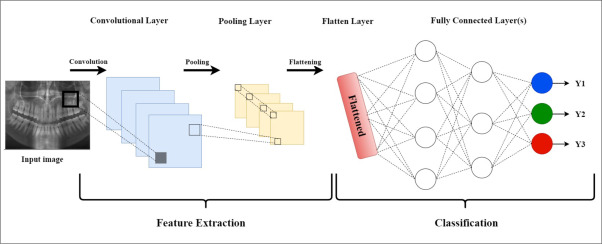
\includegraphics[width=0.8\textwidth]{figures/cnn.jpg}
    \caption{Standard block architecture and operational flow of a Convolutional Neural Network \cite{sciencedirect_cnn2026}.}
    \label{fig:cnn_arch}
\end{figure}

\subsection{Basic Principles of Object Detection in Computer Vision}
\par Object detection is a pivotal and highly challenging task in computer vision that entails two synchronous operations: identifying the presence of specific object categories within an image (classification) and delineating their exact spatial locations via bounding boxes (localization). Traditional computer vision models depended heavily on handcrafted feature extractors (such as SIFT or HOG), which lacked the robustness required for highly variable medical images. The advent of deep learning has led to an era of resilient, automated feature learning \cite{xie2023survey}.
\par Modern neural network architectures for object detection are broadly dichotomized into one-stage and two-stage detectors. One-stage detectors (e.g., YOLO variants \cite{redmon2016you}) treat object detection as a unified, single regression problem. They partition the image into a grid and simultaneously predict bounding box coordinates and class probabilities. While this single-pass architecture optimizes computational velocity and is ideal for real-time video tracking, it inherently compromises on the strict localization precision required for small objects or crowded scenes.
\par Conversely, two-stage detectors, such as the R-CNN family (including Faster R-CNN \cite{kim2020automated} and Libra R-CNN \cite{pang2019libra}), operate sequentially. The first stage generates a set of region proposals (areas of the image highly likely to contain an object), and the second stage classifies these specific regions while refining their bounding box coordinates. This rigorous methodology consistently achieves superior accuracy and handles small, difficult-to-detect objects—such as early-stage interproximal caries—exceptionally well.

\subsection{Pathological Findings in Dental Radiographs}
\par Proper comprehension of the automated detection system necessitates formal and rigorous definitions of the medical anomalies it is designed to isolate. Panoramic radiographs (orthopantomograms) and bitewing radiographs are the primary diagnostic modalities in contemporary dental practice. Due to the superimposed 3D anatomies projected onto a 2D plane, identifying minute pathologies requires substantial clinical acumen.
\par \textbf{Dental Caries:} Defined clinically as the localized destruction of susceptible dental hard tissue caused by acidic by-products from bacterial sugar fermentation. Caries detection is notoriously challenging in its incipient stages due to subtle radiographic manifestations visible only as slight radiolucencies in the enamel. High accuracy in identifying interproximal (between teeth) caries is fundamental to preventing irreversible pulp exposure \cite{schwendicke2020artificial}. In machine learning contexts, recent approaches involve consolidating heterogeneous datasets (for example, mapping distinct "Deep Caries" instances into a unified broader "Caries" class) to provide the neural network with a statistically robust number of examples, thus enhancing the generalization capabilities.

\begin{figure}[htbp]
    \centering
    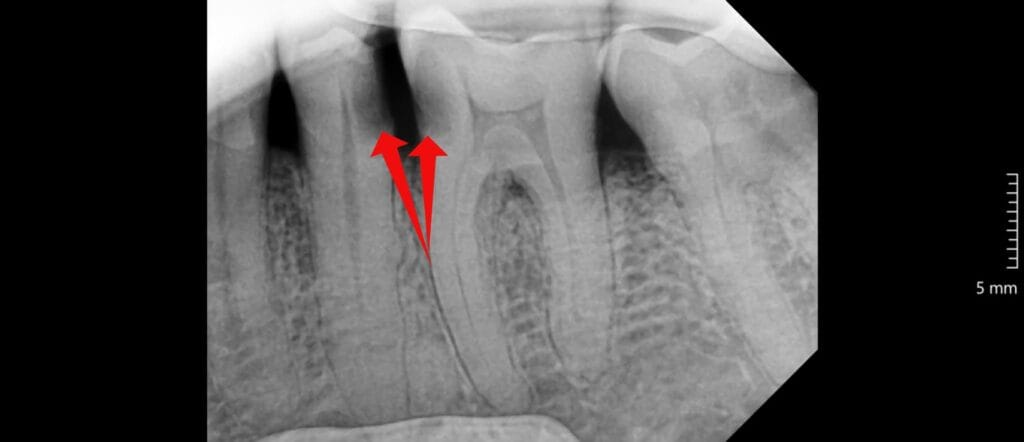
\includegraphics[width=0.6\textwidth]{figures/carie.jpg}
    \caption{Radiographic and clinical manifestation of dental caries \cite{dentalford2026}.}
    \label{fig:carie}
\end{figure}

\par \textbf{Periapical Lesions:} These are complex endodontic pathologies situated around the apex of the tooth root, manifesting predominantly as a consequence of untreated pulp necrosis. Early and accurate detection of periapical radiolucencies is highly dependent on image contrast, exposure quality, and practitioner expertise \cite{orhan2020evaluation}. Distinguishing these lesions from normal anatomical landmarks (such as the mental foramen) is a frequent point of failure for inexperienced practitioners.

\begin{figure}[htbp]
    \centering
    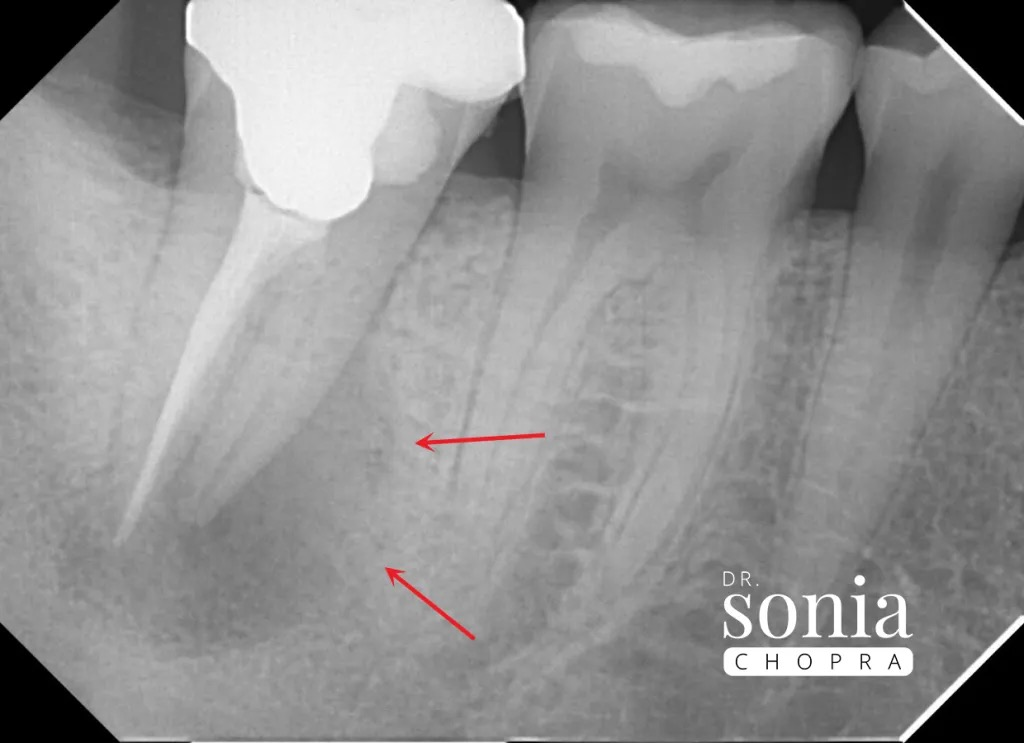
\includegraphics[width=0.6\textwidth]{figures/periapical_lesion.jpg}
    \caption{Clinical characterization and radiographic appearance of a periapical lesion \cite{chopra2026}.}
    \label{fig:periapical}
\end{figure}

\par \textbf{Impacted Teeth:} Defined as teeth that have failed to erupt fully into the functional dental arch within their expected developmental timeline constraints. Visualizing the precise angulation, root morphology, and the spatial relationship with adjacent anatomical structures (such as the inferior alveolar nerve canal) is imperative for surgical extraction planning \cite{kim2020automated}. Efficiently isolating impacted teeth as an independent diagnostic class ensures targeted reporting and avoids misclassification with normally erupting dentition.

\begin{figure}[htbp]
    \centering
    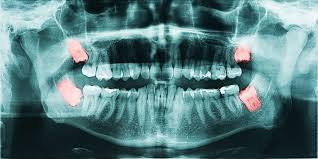
\includegraphics[width=0.6\textwidth]{figures/impacted_tooth.jpeg}
    \caption{Radiographic example of an impacted tooth obstructing adjacent structures \cite{airdrie2026}.}
    \label{fig:impacted}
\end{figure}

\section{Analysis of Current State of Research}
\label{sec:ch3_state_of_research}

\subsection{Deep Learning for Differential Diagnosis in Dentistry}
\par Research in the domain of automated dental diagnostics has gathered massive momentum, addressing the clinical necessity for objective, reproducible, and instantaneous second opinions. Hwang et al. \cite{hwang2019overview} emphasize that practitioner fatigue, cognitive bias, and varying levels of clinical experience heavily influence the interpretation of dental radiographs. Deep learning frameworks have consequently been proposed to mitigate human oversight, specifically acting to reduce the rate of false negatives (missed diagnoses) in high-throughput clinical settings.
\par The detection of dental caries remains heavily researched due to its status as the most prevalent global oral disease. Haghanifar et al. \cite{haghanifar2020dental} demonstrated that custom-designed CNNs could detect carious lesions with an accuracy metric nearing, and occasionally surpassing, expert clinician concordance. They highlighted the model's ability to identify subtle pixel density variations imperceptible to the naked human eye. Furthermore, Rahman et al. \cite{rahman2021deep} utilized a specialized deep learning framework tailored exclusively for panoramic radiographs, achieving exceptional sensitivity. However, translating these promising theoretical metrics into practical usability often encounters profound challenges, primarily driven by highly imbalanced class distributions within open-source dental datasets \cite{lee2021challenges}. Pathologies like severe periodontitis or large cysts are often severely underrepresented compared to healthy teeth, leading to biased weight distributions during network training.

\subsection{Comparison of Existing Methodological Approaches}
\par Multiple deep learning paradigms have been evaluated in recent literature for isolating dental anomalies. A standard approach has historically involved adapting existing general-purpose architectures (pre-trained on massive generic datasets such as ImageNet or MS COCO \cite{lin2014microsoft}) via transfer learning, to fine-tune the parameters on radiographic domains.
\par \textbf{Single-Stage YOLO Paradigms:} Employing single-stage architectures like YOLO (You Only Look Once) has surged in research contexts that prioritize real-time processing capabilities, such as live video feeds from intraoral cameras \cite{nguyen2023dental}. However, researchers have frequently noted that these models struggle with densely packed, small, overlapping anomalies. In dental radiographs, where multiple interproximal caries may lie millimeters apart, predicting bounded boxes directly from a grid-based regression causes significant Intersection over Union (IoU) conflicts. The Non-Maximum Suppression (NMS) algorithm often falsely suppresses valid bounding boxes under the assumption they represent duplicate predictions for the same object, thereby artificially inflating the false-negative rate.
\par \textbf{Segmentation Frameworks:} While segmentation networks (e.g., U-Net or Mask R-CNN architectures) provide precise, pixel-level boundaries which are highly advantageous for isolating morphological volumetric abnormalities (such as exact cyst volumes), their annotation overhead is debilitating. Wang et al. \cite{wang2022automated} discussed how creating comprehensive pixel-perfect segmentation datasets requires thousands of hours of expert clinical annotation. This massive barrier to entry often precludes the rapid, iterative development and fine-tuning required for scalable AI platforms.
\par \textbf{Two-Stage Faster R-CNN Adaptations:} Conversely, two-stage detectors like Faster R-CNN have proven overwhelmingly successful and highly robust for medical object detection tasks where diagnostic accuracy and the absolute minimization of false negatives cannot be subordinated to mere inference speed. Studies employing Faster R-CNN for tooth enumeration \cite{tuzoff2019tooth} and impacted tooth localization \cite{kim2020automated} reported the highest mean Average Precision (mAP) among all competing configurations. By explicitly decoupling the region proposal mechanism from the final diagnostic classification head, these architectures provide unparalleled sensitivity in identifying minute radiographic irregularities.

\begin{table}[htbp]
    \centering
    \caption{Comparative analysis of main deep learning object detection methodologies in dental imaging.}
    \vspace{0.2cm}
    \renewcommand{\arraystretch}{1.3}
    \begin{tabular}{|l|>{\raggedright\arraybackslash}p{3.6cm}|>{\raggedright\arraybackslash}p{3.6cm}|>{\raggedright\arraybackslash}p{3.6cm}|}
        \hline
        \textbf{Architecture} & \textbf{Key Advantages} & \textbf{Disadvantages} & \textbf{Optimal Clinical Use Case} \\
        \hline
        Single-Stage (YOLO) & Rapid inference speed, potential for live video monitoring. & Difficulty isolating small, overlapping objects (IoU conflicts). & Real-time assessment, basic general triage. \\
        \hline
        Two-Stage (Faster R-CNN) & Exceptional sensitivity for small pathologies, minimal false-negatives. & Slower inference, requires substantial computational power. & Asynchronous, high-accuracy diagnostic platforms. \\
        \hline
        Segmentation (U-Net) & Exact pixel-level boundaries, morphological visualization. & Massive medical annotation overhead (thousands of manual hours). & Volumetric tracking (e.g., severe cysts). \\
        \hline
    \end{tabular}
    \label{tab:architecture_comparison}
\end{table}

\section{Technological Infrastructure and Architectures}
\label{sec:ch3_technologies}

\par The synthesis of a functional clinical platform requires both theoretically rigorous machine learning architectures and highly optimized software engineering frameworks. The platform constructed for this thesis relies extensively on the Faster R-CNN architecture, supercomputing training infrastructure, an asynchronous backend, and a modern Generative AI pipeline.

\subsection{Faster R-CNN: A Deep Dive into Two-Stage Detection}
\par The foundational algorithm selected for detecting pathological findings is Faster R-CNN. As an advanced two-stage detector, Faster R-CNN dramatically redefined computer vision standards by eliminating the reliance on external algorithmic region proposals, instead embedding this capability directly within the neural network via the Region Proposal Network (RPN).

\begin{figure}[htbp]
    \centering
    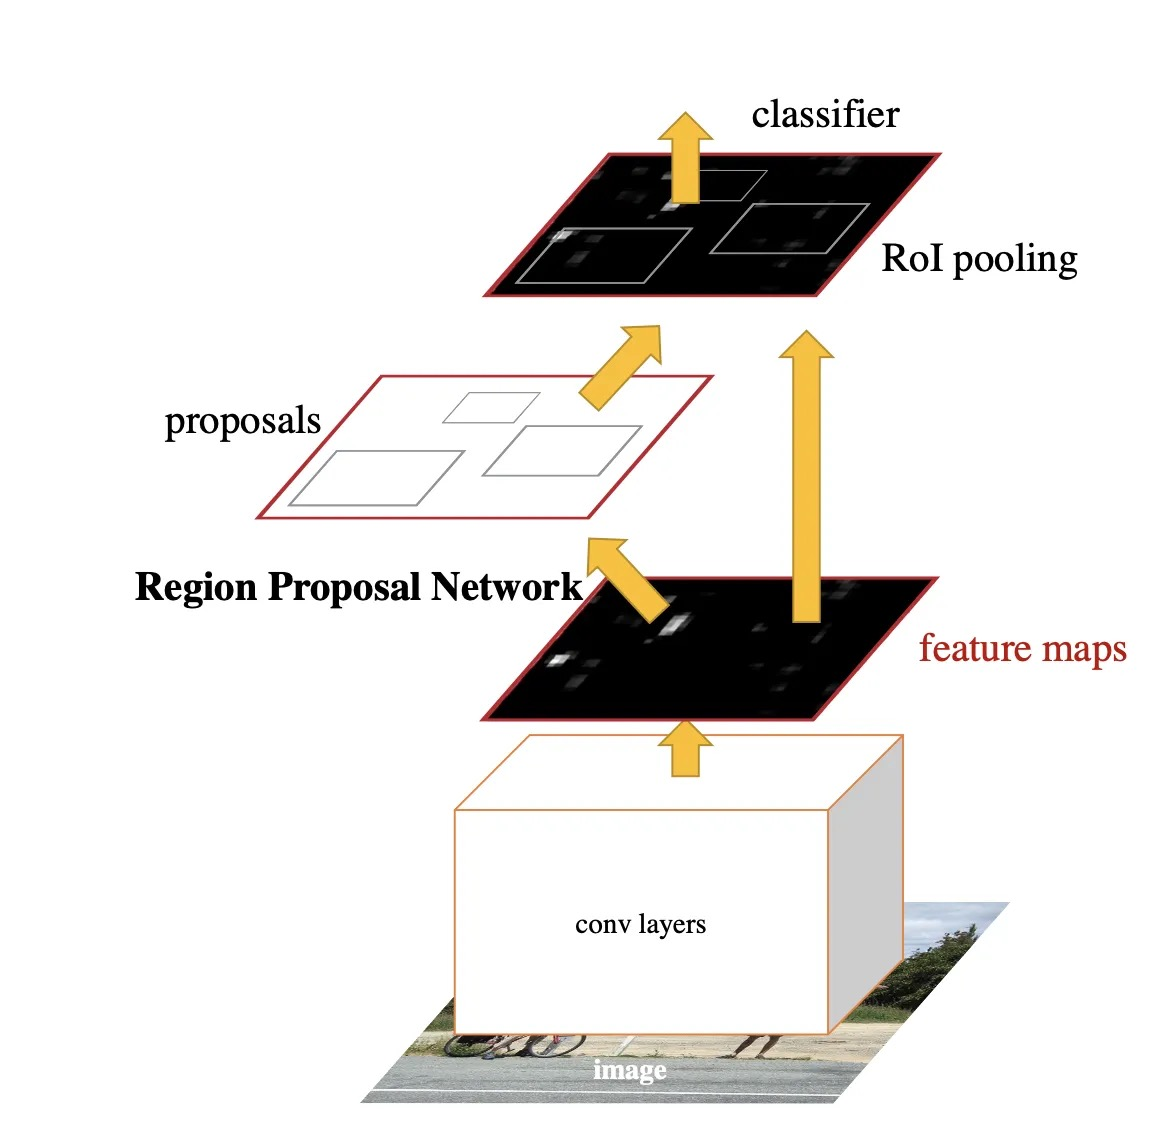
\includegraphics[width=0.85\textwidth]{figures/fasterrcnn.jpg}
    \caption{Detailed architectural schema of Faster R-CNN illustrating the Region Proposal Network (RPN) and the final classification layers \cite{cloudfactory_faster2026}.}
    \label{fig:faster_rcnn}
\end{figure}
\par \textbf{The Feature Extraction Backbone:} In the initial phase, the raw radiological image is passed through a convolutional backbone (in this implementation, utilizing variants such as ResNet-50) to extract a highly condensed, dense, structural feature map. This backbone acts as the visual cortex of the platform, identifying the underlying gradients and textures of the dental anatomy.
\par \textbf{The Region Proposal Network (RPN):} The key innovation of Faster R-CNN is the RPN. The RPN slides a theoretical spatial window across the entirety of the dense feature map generated by the backbone. At each sliding-window location, the network predicts multiple region proposals simultaneously using reference boxes known as "anchors." Anchors are predefined bounding boxes of varying scales and aspect ratios (for example, tall and narrow for a tooth root, or small and square for a carious lesion). The RPN computes two distinct outputs for each anchor: an "objectness" score (a probability reflecting whether the anchor bounds a relevant anomaly or mere background noise) and the architectural coordinate regressions modifying the anchor box to fit the anomaly securely.
\par \textbf{Region of Interest (RoI) Pooling:} Generating proposals of varying sizes poses a massive challenge for subsequent classification layers that require fixed-dimension inputs. RoI Pooling acts as the bridge. It extracts features from the backbone's feature map corresponding to each proposed region and max-pools them into a uniform, fixed-length feature vector regardless of the original proposal's dimensions \cite{xie2023survey}.
\par \textbf{Final Classification Head:} Finally, these normalized feature vectors are fed into two parallel fully connected (dense) layers. The first layer outputs the final classification label utilizing a Softmax function (specifying if the object is Caries, an Impacted Tooth, or a Periapical Lesion), while the second layer outputs a final, highly refined set of bounding box coordinates. This rigorous computational verification ensures that subtle diagnostic features are exhaustively evaluated.

\subsection{Generative AI for Automated Treatment Planning}
\par A major limitation of traditional computer vision models in the medical domain is that they provide purely observational outputs (e.g., bounding boxes and class labels) without actionable clinical synthesis. To bridge the gap from automated observation to proactive clinical assistance, this research integrates a secondary, highly advanced Artificial Intelligence component: a Generative AI API based on Large Language Model (LLM) architecture.
\par Once the Faster R-CNN model concludes the inference step and outputs its array of bounding boxes, anomaly classifications, and confidence scores, the platform structures this raw data into a structured context object (e.g., a formal JSON schema). This structured data acts as an intelligent prompt parameter. It lists the exact pathologies detected, their anatomical locations (if correlated with an enumerated tooth array), and the severity implied by the confidence metrics.
\par This formalized diagnostic matrix is securely transmitted via an API to a pre-prompted Generative LLM. The LLM acts as an expert clinical reasoning engine. By analyzing the combination of recognized pathologies, the LLM utilizes its vast corpus of contemporary dental literature to automatically synthesize a step-by-step, actionable treatment plan. For instance, if the object detection model identifies deep interproximal caries alongside a periapical radiolucency on an adjacent tooth, the Generative API dynamically formulates a comprehensive strategy. The strategy ranks interventions by clinical urgency, explicitly recommending endodontic therapeutic evaluations prior to scheduling restorative fillings, and outlines post-operative monitoring advice. This integration transforms the platform from a mere detection overlay into a comprehensive, intellectual diagnostic assistant that actively guides the clinical workflow.

\subsection{Cloud Infrastructure and Hyper-Accelerated Training Methodology}
\par Executing the training of a heavy two-stage architecture fundamentally requires massive computational power to process millions of tensorial backpropagations accurately. 
\par \textbf{NVIDIA A100 GPU computing (Google Colab):} To parallelize these exhaustive tensorial computations across the required 100-epoch training phase, execution was deployed leveraging the ultra-high-performance NVIDIA A100 Tensor Core GPU architecture hosted on the Google Colab Pro cloud infrastructure. The A100 architecture offers monumental improvements in memory bandwidth and floating-point operations per second (FLOPS). This distributed cloud infrastructure was unequivocally instrumental in overcoming the severe local computational bottlenecks that would have critically hindered model convergence on standard consumer hardware.
\par \textbf{Datatset Engineering:} To optimize the Faster R-CNN's performance logic, profound dataset engineering was executed prior to cloud training. By strategically compiling and remapping heavily divergent datasets (specifically merging the Mendeley radiographic repository with the Dentex dataset), the model was fed a vast, highly diverse visual corpus. Crucial class remapping procedures were undertaken; distinguishing "Deep Caries" from "Caries" often introduces unnecessary noise for bounding box regression. Unifying them into a singular "Caries" class significantly concentrated the network's learning threshold. Simultaneously, isolating "Impacted Teeth" as a strictly standalone class drastically empowered the RPN to converge efficiently, predicting class probabilities with maximal clinical utility and minimal contextual confusion.

\subsection{Web Platform Engineering and User Interfaces}
\par Transitioning the fully trained Faster R-CNN model and the Generative AI treatment planner from academic scripts to a functional web dashboard relies on robust modern engineering frameworks capable of managing immense asynchronous workloads.
\par \textbf{Backend Architecture (FastAPI/Python):} Python maintains a monopoly over deep learning implementations due to the absolute ubiquity of the PyTorch mathematical ecosystem. The modern framework FastAPI was strategically selected as the core infrastructural backend over legacy monolithic systems like Django or Flask. FastAPI is distinguished by its native asynchronous execution capabilities and intrinsic support for strict data validation utilizing Pydantic models. This permits optimized, non-blocking background processing of heavy DICOM or JPEG image uploads. It securely executes the Faster R-CNN tensor evaluations, subsequently triggers the Generative AI API calls in parallel, and serializes the fused coordinate and treatment plan payloads into JSON formats with near-imperceptible latency.
\par \textbf{Frontend Application (React.js):} The client-facing user interface is engineered utilizing React, a declarative and component-based JavaScript library focused heavily on virtual Document Object Model (DOM) rendering optimization. React's profound state management architectures facilitate a smooth, uninterrupted user experience. It seamlessly manages asynchronous HTTP requests, orchestrating loading states while the server models are triggered. Most importantly, it rapidly renders dynamic, interactive SVG-based bounding boxes precisely overlaid across the uploaded dental radiograph coordinates, all alongside displaying the comprehensive, LLM-generated treatment recommendations without necessitating a disruptive browser refresh.

\subsection{Ultimate Justification of Methodological Selection}
\par The specific amalgamation of technological instruments outlined above was meticulously selected to unequivocally address performance and usability gaps prevalent in current dental informatics. While prioritizing sheer real-time inference speed (measured in milliseconds) may be technically impressive in autonomous driving environments, clinical dentistry predominantly involves static frame analysis where zero-tolerance for diagnostic false negatives unequivocally supersedes processing velocity.
\par The selection of the two-stage Faster R-CNN over single-stage regression models like YOLO is biologically and scientifically justified by the stringent requirement to identify minuscule, complex pathologies. Faster R-CNN's RoI Pooling guarantees that overlapping anomalies receive independent, rigorous evaluation, yielding massively superior operational sensitivity. A clinical practitioner can comfortably accommodate an uploading and remote processing latency of two to three seconds, provided that the ensuing anatomical overlay boundary is flawlessly accurate.
\par Integrating this state-of-the-art vision model with an innovative Generative AI treatment planner completely redefines the scope of the software. Rather than abandoning the clinician at the interpretation phase, the platform acts continuously to relieve cognitive load, mapping the recognized visual detriments directly into structured clinical interventions. Finally, pairing these powerful AI pipelines entirely within a FastAPI and React distributed infrastructure provides a resilient, massively scalable application that successfully achieves all rigorous academic and diagnostic objectives established for this thesis.
